\chapter{Overview}

\todo{briefly explain this section}


\section{The Raspberry Pi 3 Cluster} \label{pi4cluster}

\todo{talk and show a picture of the physical testbed}

\begin{table}[H]
    \centering
    \begin{tabular}{ |p{4cm}||p{2cm}|p{3cm}|p{2cm}|p{2cm}|p{2cm}|  }
        \hline
        \multicolumn{6}{|c|}{\textbf{Raspberry Pi 3 Specifications}} \\
        \hline
        CPU & RAM & NICs & Storage & USB & OS\\
        \hline
        Broadcom BCM2837B0 \newline Cortex-A53 (ARMv8) 64-bit SoC \newline 1.4GHz, Quad-core &
        1 GB LPDDR2 SDRAM &
        Gigabit Ethernet over USB 2.0 \newline \newline Dual IEEE 802.11ac WiFi, Bluetooth 4.2 &
        32GB Micro-SD &
        4 USB 2.0 ports &
        Raspbian Buster (Linux) \newline or \newline FreeBSD\\
        \hline
    \end{tabular}
    \caption{The hardware specifications of Raspberry Pi 3.}
\end{table}

\todo{move OS to another table containing network setup}

\section{Network Topology} \label{topology}

\todo{talk and show a diagram of the network topology}

\begin{figure}[H]
    \centering
    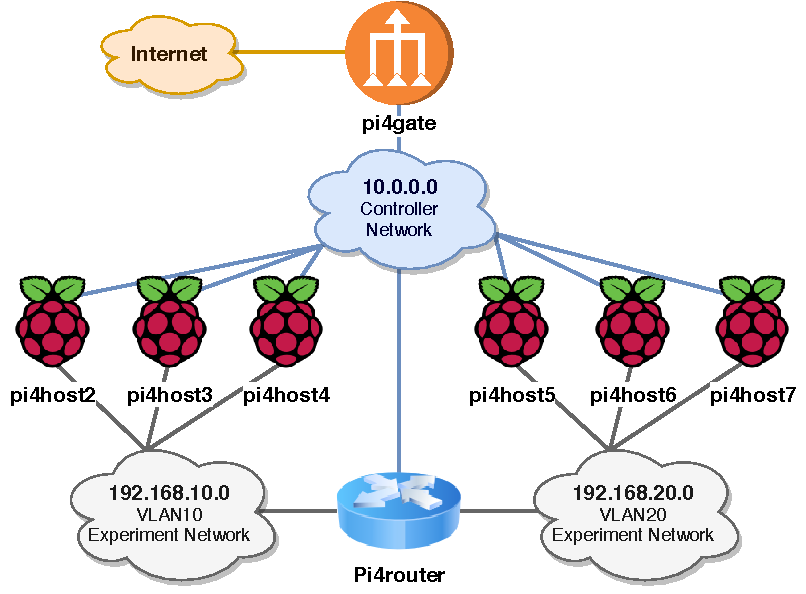
\includegraphics[width=0.6\linewidth]{network_topology}
    \captionsetup{width=0.6\linewidth}
    \caption{The logical network topology for the Raspberry Pi 3 cluster testbed. \todo{maybe update diagram to account for virtual interfaces and VLANs}}
    \label{fig:network_topology}
\end{figure}